%
% Omigost Project
%
% MIT License
% Copyright 2018
%
% Piotr Styczyński     (University of Warsaw)
% Michał Balcerzak     (University of Warsaw)
% Michał Ołtarzewski   (University of Warsaw)
% Gor Safaryan         (University of Warsaw)
%
% Permission is hereby granted, free of charge, to any person obtaining a copy of this software and associated documentation files (the "Software"),
% to deal in the Software without restriction, including without limitation the rights to use, copy, modify, merge, publish, distribute, sublicense,
% and/or sell copies of the Software, and to permit persons to whom the Software is furnished to do so, subject to the following conditions:
%
% The above copyright notice and this permission notice shall be included in all copies or substantial portions of the Software.
%
% THE SOFTWARE IS PROVIDED "AS IS", WITHOUT WARRANTY OF ANY KIND, EXPRESS OR IMPLIED, INCLUDING BUT NOT LIMITED TO THE WARRANTIES OF MERCHANTABILITY,
% FITNESS FOR A PARTICULAR PURPOSE AND NONINFRINGEMENT. IN NO EVENT SHALL THE AUTHORS OR COPYRIGHT HOLDERS BE LIABLE FOR ANY CLAIM,
% DAMAGES OR OTHER LIABILITY, WHETHER IN AN ACTION OF CONTRACT, TORT OR OTHERWISE, ARISING FROM,
% OUT OF OR IN CONNECTION WITH THE SOFTWARE OR THE USE OR OTHER DEALINGS IN THE SOFTWARE.
%
%
%

% Add option for language formatting en/pl
\documentclass[licencjacka,en]{thesisclass}
\usepackage{standalone}
\usepackage{import}
\usepackage{graphicx}
\usepackage{grffile}
\usepackage{svg}
\usepackage{calc}
\usepackage[backref=true,                %
hyperref=true,               %
firstinits=true,             %
indexing=true,               %
url=false,                   %
style=alphabetic,            %  style=debug, alphabetic
backend=biber,               %
doi=false,
texencoding=utf8,
bibencoding=utf8]{biblatex}

\addbibresource{src/thesis.bib}
\usepackage{biblatex}
\addbibresource{src/thesis.bib}

% Authors of the thesis:
\autor{Piotr Styczyński}{386038}
\autori{Michał Balcerzak}{385130}
\autorii{Michał Ołtarzewski}{382783}
\autoriii{Gor Safaryan}{381501}

\title{AWS Cost Optimization Tool}
\titlepl{Narzędzie do Optymalizacji Kosztów AWS}

% The main degree
\kierunek{Computer Science}

% The thesis supervisor
\opiekun{dr Janina Mincer-Daszkiewicz\\
Instytut Informatyki\\
}

% Date in format <month> <year>
\date{February 2019}

% Doctrine of classification as it states the Socrates-Erasmus:
\dziedzina{
11.3 Informatics, Computer Science\\
}

% TODO
% Subject classification due to ACM
\klasyfikacja{D. Software}

% Keywords list
\keywords{AWS, Amazon Web Services, cloud computing, cost optimization, cost management}

% TODO
% Place for custom definitions and environments
\newtheorem{defi}{Definicja}[section]

% End of definitions

\usepackage{lmodern}

\begin{document}
    \maketitle

    % Brief for the first page (short abstract)
    \begin{abstract}
        %
% AWS Cost Optimization Tool Project
%
% MIT License
% Copyright 2018
%
% Michał Balcerzak     (Univeristy of Warsaw)
% Michał Ołtarzewski   (Univeristy of Warsaw)
% Piotr Styczyński     (Univeristy of Warsaw)
% Gor Safaryn          (Univeristy of Warsaw)
%
% Permission is hereby granted, free of charge, to any person obtaining a copy of this software and associated documentation files (the "Software"),
% to deal in the Software without restriction, including without limitation the rights to use, copy, modify, merge, publish, distribute, sublicense,
% and/or sell copies of the Software, and to permit persons to whom the Software is furnished to do so, subject to the following conditions:
%
% The above copyright notice and this permission notice shall be included in all copies or substantial portions of the Software.
%
% THE SOFTWARE IS PROVIDED "AS IS", WITHOUT WARRANTY OF ANY KIND, EXPRESS OR IMPLIED, INCLUDING BUT NOT LIMITED TO THE WARRANTIES OF MERCHANTABILITY,
% FITNESS FOR A PARTICULAR PURPOSE AND NONINFRINGEMENT. IN NO EVENT SHALL THE AUTHORS OR COPYRIGHT HOLDERS BE LIABLE FOR ANY CLAIM,
% DAMAGES OR OTHER LIABILITY, WHETHER IN AN ACTION OF CONTRACT, TORT OR OTHERWISE, ARISING FROM,
% OUT OF OR IN CONNECTION WITH THE SOFTWARE OR THE USE OR OTHER DEALINGS IN THE SOFTWARE.
%
%
%

The thesis describes the design and implementation process, in-depth system and code architecture
as well as used communication protocols, storing methods and other internals of the AWS Cost Optimization System.
    \end{abstract}

    \chapter*{Contents}

    \begin{enumerate}
        \item Introduction
        \begin{enumerate}
            \item [1.1] Overview
            \item [1.2] Aim of the thesis
            \item [1.3] Structure of the thesis
            \item [1.4] Contribution of each author
        \end{enumerate}
        \item Problem statement
        \begin{enumerate}
            \item [2.1] Motivation
            \item [2.2] Overview of exisiting solutions
            \item [2.3] Our solution
        \end{enumerate}
        \item Project development
        \begin{enumerate}
            \item [3.1] Version control
            \item [3.2] Continuous integration
            \item [3.3] Communication
            \item [3.4] Workflow
        \end{enumerate}
        \item Tool for AWS cost optimization
        \begin{enumerate}
            \item [4.1] Overall architecture
            \item [4.2] Technology stack
            \item [4.3] Data models
            \item [4.4] Views and design
            \item [4.5] API
            \item [4.6] Communication integration
            \item [4.7] Configuration
        \end{enumerate}
        \item Summary
        \item [A] Deployment and integration guide
    \end{enumerate}

    \chapter{Introduction}

    % 
\includegraphics[width=\textwidth*\real{0.4}]{imgs/logo.png}

    \section{Overview}

    Cloud computing has become recently one of the most important paradigm shifts in the area of real world software engineering.
    It has reshaped the whole process of how applications are developed and reduced the amount of upfront
    investment required to start an internet business. While commercial cloud computing services were first offered
    in 2006 by Amazon Inc, the original idea and preliminary implementation traces back to Multics OS developed by MIT,
    GE and Bell Labs. However the idea of time-sharing systems that was the ancestor of further cloud
    concept was widespread in 60ies~\cite{Markus}.

    The term “Cloud computing” can refer to every layer of application stack:
    hardware, hosting platform, software and even to a single function.
    Cloud computing refers to both the applications delivered as services over the Internet and
    the hardware and systems software in the data centers that provide these services.
    The services themselves have long been referred to as Software as a Service (SaaS)~\cite{Armbrust}.
    Generally speaking cloud can be perceived as a shared pool of computer resources such as computing capacity,
    transient and persistent memory, which can be acquired or released on demand.
    The undisputed power of cloud computing constitutes in its elasticity and granularity: it allows users to ask for hundreds of computers for only 5 minute usage which
    are shipped during several minutes.
    Such services are usually offered over remote network connection and users are billed
    for the portion of the resources they have used.
    Depending on the cloud infrastructure type the payment models can be different~\cite{Laatikainen},
    but the common spendings are associated with data storage, data transfer, and computing timeshare.

    Nowadays the industry increasingly relies on cloud technologies. More and more companies start or move their products to cloud environment.
    Unfortunately it comes with additional financial costs imposed by cloud providers.
    In order to make business profitable companies try to reduce amont of money they are supposed to pay to the minimum. Despite different solutions, like employing specific cloud cost optimization team, more and more firms decide to benefit from dedicated software, which is supposed to help manage and optimize their cloud usage. It is not easy to chose the right tool having that many choices.

    There are some notable solutions of AWS cloud optimization problem -- \textit{AWS Cost Explorer} and \textit{AWS Cost Management}, \textit{Cloudability}, \textit{Apptio} and others widely used nowadays. In spite of that fact there is still place for new tools targeting omitted types of clients or wrapping and bundling the greatest features from exisiting ones.

    \section{Aim of the thesis}

    The primary objective of the thesis is to create a tool complementing existing solutions used in cloud cost optimisation. We focuse on Amazon Web Services platform maintained by Amazon as it is one of the most commonly used.
    In our tool, called \textit{Omigost}, we will try to target small/middle sized companies creating simple and easy to use software with flexible configuration options.

    \section{Structure of the thesis}

    The thesis is structured as follows. In Chapter 2 we describe the problem of cloud cost optimization with additional description of selected existing solutions. Then, in Chapter 3 we present our solution in detail. We mention, among others, whole system architecture, API and configuration. Finally, in Chapter 4 we sum up the whole thesis. In Appendix A we describe how to introduce our solution in a company.

    \section{Contribution of each author}

    It is important to mention that each author worked to some extent on every part of the thesis. However authors contributed mainly to the following parts:

    \begin{itemize}
        \item Michał Ołtarzewski
        \begin{itemize}
            \item Software development process management
            \item Design of backend architecture
            \item Backend part implementation
        \end{itemize}
        \item Michał Balcerzak
        \begin{itemize}
            \item Research of existing solutions
            \item Design of backend architecture
            \item Backend part implementation
        \end{itemize}
        \item Piotr Styczyński
        \begin{itemize}
            \item Design and prototype of visual part of tool
            \item Frontend part implementation
        \end{itemize}
        \item Gor Safaryan
        \begin{itemize}
            \item Research of AWS APIs and SDKs
            \item Design of backend architecture
            \item Backend part implementation
        \end{itemize}
    \end{itemize}

    % \subsection{Cloud resources}
    %
    % Cloud computing has introduced 3 new aspects which are radically different from a traditional
    % computing paradigm in terms of hardware infrastructure.
    % The availability of practically infinite on demand computing resources,
    % which allows users to deploy applications without any kind of resource planning.
    % The elimination of massive initial financial commitment, therefore allowing small companies to increase
    % their hardware usage proportional to their needs.
    % The ability to granularly allocate computing resources on any kind of timeframe
    % (from minutes up to days etc.), as well as the ability to release them as there is no more need.
    %
    % Depending on the service offered by the provider we differentiate 3 main models of cloud computing:
    %
    % \begin{enumerate}
    %     \item Infrastructure as a service (IAAS).
    %     \item Platform as a service (PAAS).
    %     \item Software as a service(SAAS).
    % \end{enumerate}
    %
    % % TODO discuss double dash vs triple dash
    % \subsection{IAAS -- Infrastructure as a service}
    %
    % In such form of service, the provider allocates an instance of virtual machine for the client
    % and ensures that minimal building blocks for the IT infrastructure are present:
    % network, storage, computing capacity, load balancer, VLAN etc.
    % Usually providers of such services run pools of hypervisors such as Xen, VMware, QEMU etc which host and manage
    % those virtual machines. From the user perspective it usually looks like a command line interface
    % through which user has full control over the allocated virtual machine. Some of the well known
    % services are Amazon EC2, Google Compute Engine, Microsoft Azure IAAS.
    %
    % \subsection{PAAS -- Platform as a service}
    %
    % Platform as a service alleviates the need for the developers to manage the operating system and
    % provides programming language specific execution environment as well as the underlying structure
    % (hardware, network, storage etc). This adds another layer of convenience over IAAS making the deployment
    % and the development of applications much more fluent process. While users benefit from the automatic software maintenance,
    % OS security patches etc, they also lose full control over the virtual machine instances. AWS Elastic Beanstalk, Heroku
    % and Google App Engine are some of the most popular PAAS services.
    %
    % \subsection{SAAS -- Software as a service}
    %
    % This form of service takes control of every layer of application and the user has nothing to do with
    % the underlying infrastructure. This is by all means one of the most popular form of cloud computing as
    % it might not require any kind of technical background to be used. Examples of SAAS services are Google
    % Cloud Vision, Google Docs, Microsoft Office 365.

    \chapter{Problem statement}

    \section{Motivation}

    As there are plenty of various billing models for cloud services~\cite{GLaatikainen},
    the effective management of them became a tough problem.
    The ease of resource allocation led to situation when tracking tiniest details of billings is an unaffordable challenge.

    The tooling that exists is targetting wideworld-scale companies that are able to require expensive licenses and hire cost-optimization teams.
    The software as it is in case of Cloudability is too complex for average user and does not provide easy way to incorporate custom business flows into the tool.
    Amazon, as one of the leading cloud providers, offers different tools for exploration of expenses. Most commonly used options are either their public APIs~\cite{AWSCostManagement} or specific SDKs supporting lots of languages.
    Unfortuantely previously mentioned tools are rather simple and do not satisfy all the needs of potential clients.

    The common case that is unresolved is the distribution of research and development resources.
    We observed that there exists no tool that would support request for resources of individual worker with regards to custom management propagations as specified by client bussiness model.
    Cloudability~\cite{CloudabilityAlerts} offers simple alerts, but they lack Slack support and beforementioned propagation abilities.

    There exists an obvious gap in the market, that our solution, \textit{Omigost}, will try to cover. Having one versatile tool removes the need for using few detached pieces of software. The most important aspects of our tool are intuitive interface and different types of user notifications, which highly increases spendings clarity and helps in decisions connected to costs cutting. We hope it will allow companies to focus more on providing value to their clients having lower costs in the same time.
    Problem we would like to solve is lack of the tool that has simultaneously the following features:
    \begin{itemize}
        \item Free and Open Source
        \item Easy cloud management without complex knowledge
        \item Intuitive interface for individual workers to request resources
        \item Notifications for cost surpassing and redundant resources
        \item Manage notification well -- only significant alerts
        \item Highly configurable and flexible
        \item Integration with communication via Email and Slack
    \end{itemize}

    \section{Overview of exisiting solutions}

    Businesses that rely upon cloud services often reach a point where resources
    they are using up gradually become less and less manageable.
    As the problem is well known to the cloud market, both Amazon and other third-party companies made attempts
    to fulfill these needs by creating custom software fitting certain roles in optimizing AWS expenses that include:

    \begin{enumerate}
        \item Configuring budget limits and alerting users when they are exceeded
        \item Instance alerting management
        \item Cost analytics
    \end{enumerate}

    Some of the most prominent tools currently available on the market that improve resource management experience for AWS cloud are described in the following sections. Every description is supposed to show key features crucial for cost optimization.

    \subsection{AWS Budgets}

    AWS Budgets\cite{AWSDocs} is a part of Amazon Web Services that allows to set limits of a certain types
    that apply to a chosen period of time.
    When a limit is either exceeded, close to be exceeded or is forecasted to exceed the configured threshold
    before the end of that period, the administrator of that account is notified by email.
    Types of resources one can put this kind of a budget on include:

    \begin{enumerate}
        \item Money spent in total or on a certain type of machines.
        \item Utilisation of selected services.
        \item Utilisation or coverage of reserved instances.
    \end{enumerate}

    \subsection{AWS Cost Explorer and AWS Cost Management}

    AWS Cost Explorer\cite{CostExplorer} enables access to all budget data.
    User can define and generate custom reports in a form of a data chart spanning a selected time interval with chosen time granularity of the samples.
    % https://aws.amazon.com/aws-cost-management/aws-cost-explorer/
    AWS Cost Explorer is also a basis for AWS Cost Management, which is basically a set of predefined reports that form an easily accessible dashboard.
    % https://aws.amazon.com/aws-cost-management/

    \subsection{Cloudability}

    Atlassian's Cloudability\cite{Cloudability} delivers a budget system functionality analogous to AWS Budgets
    along with tools for predicting future spendings and presenting the real cost of AWS resources in utilisation.
    In comparison to Amazon's native tools Cloudability also allows management of multiple accounts in the same time. It saves effort of having to set up budgets separately in every owned account.

    \subsection{Apptio}

    Apptio\cite{Apptio} provides a set of tools that mainly focuses on analysis of expenses and their forecasts,
    managing them collaboratively, and planning future ones.
    They expose features that make it easier to discover underutilized resource,
    compare spendings with a database of similar benchmarks,
    organize resources into groups to make reports even clearer,
    and offer other useful management utilities.

    \subsection{Stax.io}

    Stax.io's\cite{Stax.io} main focus is to provide insight about cost, wastage, compliance and cloud quality.
    It can analyse how cloud resources are used, measure quality of the way cloud is utilized,
    set up checks for business-compliance of our cloud with several standards
    and give customized advice on what could be optimized to reduce wastage,
    while also allowing for creation of custom views of data.
    Basic tools for budgeting instances, accounts, tags and more, monthly or annually,
    and configuring overspend alerts are also available there.

    \subsection{SnowSoftware}

    SnowSoftware's toolset, alongside fulfilling some of the more specific usecases
    like optimizing usage of software from SAP Software Solutions or optimizing and managing software licenses,
    also has tools that are dedicated to optimizing cloud costs.

    Snow for SaaS attempts to give a holistic view about application usage including, among others,
    how SaaS applications are used on cloud and whether there are zombie virtual machines~\cite{SnowSaaS}.

    Snow Automation Platform suggests approach based on automated and preconfigured provision of resources.
    By pre-giving those resources a decommission date one can avoid issue of zombie instances.
    It is also possible to preconfigure budgets and schedule machine starts and stops to further optimize costs~\cite{SnowBlog}.

    \subsection{Conclusions}

    Using resources available to us, we concluded that most of the competing tools available on the market
    fail to provide both instance budgeting and machine termination automation.
    A number of them also puts most of their emphasis on analysing usage data rather than
    helping with instance management.
    From tools listed above, Snow Automation Platform is the only one that features both budgeting and automating
    machine termination and stopping.
    However, it's approach is not to straightforwardly manage already existing machines,
    but rather to automate their provisioning.

    \section{Our Solution}

    TODO

    % TODO Begin chapter 3 with showing our product and then comparing with the conclusions above


    \chapter{Project development}

    In this section we will describe the way we developed the application -- managament and organization of work along with supporting tools.

    TODO

    \section{Version control}

    During development as our version control system we use Git and whole code repository is hosted on GitHub. We have chosen this particular service because of a few reasons.

    First of all GitHub\cite{GitHub} is one of the most popular Git hosting service and also has one of the biggest open source communities. It is quite important if we consider possibility of future development of our tool even after finishing this thesis.

    The second reason is integration with lots of useful applications. It is easy to use it with different services improving development process like TravisCI\cite{TravisCI} and Slack\cite{Slack}.

    Last but not least, GitHub has built in issue tracker. It can be highly customised and makes project management easier. We created dashboard divided into a few sections, which separate tasks in different stages of development. Everything is automated -- depending on actions performed by users like Pull Requests issues are moved between sections. In order to help prioritize tasks we introduced issues tagging system.

    \section{Continuous Integration}

    For Continuous Integration we use hosted service -- TravisCI. It allows us to make sure new changes we introduce are compliant with the rest of our codebase. There are two reasons we have chosen this service: it is easy to configure using only one YAML file inside repository and it is free for open source projects. After every code submission, at the beginning TravisCI performs Smoke Tests trying to build the project and check whether it runs or not. Successful build is followed by both backend and frontend tests.

    \section{Communication}

    All of the communication happens via Slack. It is a platform allowing team members to communicate without use of email or group SMS. Various channels can be created there, with persistent messages history both public and private. There is also possibility to reach out to every member directly if needed. We use Slack due to the fact it is free and integrates easily with GitHub.

    \section{Organization of work}

    We work in iterations that last around one month. At the beginning we define and create new issues. During the iteration everyone chooses desirable task, completes it and makes corresponding Pull Request in GitHub. At the end we discuss our overall progress and plan next steps.

    In order to let a new feature become part of the repository it has to be accepted. It means that Pull Request has to pass Continuous Integration system build and be approved by one of the reviewers.
    Every issue is solved in a separate branch and every PR is merged directly to the master branch, which allows us to group all commits that are part of one feature or issue.

    \section{Contact with client company -- Sumo Logic}

    TODO (not sure if right title)


    \chapter{Tool for AWS cost optimization}

    In this chapter we will describe the whole application -- \textit{Omigost}.

    \section{Overall architecture}
    Our solution utilizes an architecture that can be briefly visualized with the following figure:

    \begin{figure}[!htb]
      \center{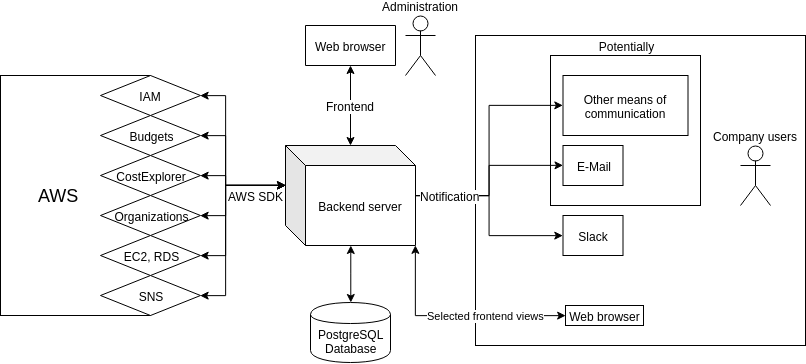
\includegraphics[width=\textwidth] {imgs/arch_diagram.png}}
      \caption{\label{fig:arch-diag} Draft diagram of the tool architecture}
    \end{figure}

    The architecture we use can be described as a traditional client-server architecture.
    Actors make requests over the HTTP protocol to our system with a web browser using our frontend client application
    served by our server or, alternatively, from any kind of a storage service like, for example, Amazon's S3.
    Those requests are then handled by a backend application of all requests is handled by a central server machine.
    During the handling process our application utilizes both a local instance of a PostgreSQL relational database
    and a connection with selected Amazon Web Services via a SDK library.
    Additionally, end users are notified about budget or instance events related to their cloud activity through Slack.

    \subsection{Role of AWS cloud services}
    Connecting with Amazon's cloud services not only allows the application to access instance and spending data
    that is crucial to be able to fulfill the business requirements,
    but many of them also solve many of the problems we would otherwise have to solve ourselves - resulting
    in time saved and a codebase that is more concise and easier to maintain.

    Services that are used in the project and their respective roles in it are as follows:
    \begin{itemize}
        \item Identity and Access Management (IAM) -- provision of the main Amazon account ID that is used in other services,
        \item Organizations -- insight into structure of the Organization used by the company, including listing accounts,
        \item Budgets -- configurable spending watches that trigger a SNS notification whenever a budget limit is or is going to be exceeded,
        \item SNS -- alert notifications for backend that let it know about spendings events,
        \item Cost Explorer -- data for graph visualizing spendings in frontend,
        \item EC2/RDS -- information about state of instances running on the account.
    \end{itemize}

    TODO at the end of the project - check if any other "sublibraries" were used and/or if any other usecases emerged

    \subsection{Backend}

    Backend is the main agent of our application's functionalities.
    It is responsible for fetching or receiving data from either of other connected resources, parsing it and taking appropriate actions.
    Some of its more important tasks include:
    \begin{itemize}
        \item receiving SNS budget alert notifications and notifying appropriate users via Slack,
        \item fetching and providing raw data for the frontend so it can be displayed to the user,
        \item receiving configuration or data modification requests and adjusting the application environment components to fulfill them,
        \item checking machine state on preconfigured times and notifying users about possible instance optimizations.
    \end{itemize}

    \subsection{Frontend}
    Frontend is a web application that allows our user to see and alter the state of our application using a graphical user interface (GUI).
    Its main roles are to:
    \begin{itemize}
        \item request and parse raw data from backend into visual representations of it,
        \item provide an interface for the user,
        \item translate the interface clicks to appropriate backend requests and display the results of those requests.
    \end{itemize}

    \section{Technology stack}

    \subsection{Frontend}

    TODO

    \subsection{Backend}

    Core of the backend is \textit{Java 8}. We have selected this programming language because most of us were familiar with it. Also this language has huge community and lots of useful libraries and frameworks.

    For creation of the whole backend service we have chosen Spring\cite{Spring} framework. It is currently one of the most common choices. Spring allows to build web applications imposing usage of design patterns like Model-View-Controller and Dependency Injection. It helps to keep code easily testable and well organized. Additionaly it provides various features out of the box, which speeds up development process.

    Gradle\cite{Gradle} is responsible for build and dependencies management. It is easy to use with various IDEs and flexible configuration. The main competitor of Gradle is Maven so obviously we considered both. Gradle turned out to be better in terms of performance and usage convenience.

    For data persistance we have picked PostgreSQL database. Relational database enforces having strictly defined data model with validation. Performance is not an important aspect for us so there was no need for other types of databases. PostgreSQL is great open source database with strong data integrity and fault-tolerancy guaranties. Furthermore AWS lets set up PostgreSQL instance with just few clicks with automaticaly configured parameters for optimal performance.

    In our application we use the following libraries:
    \begin{enumerate}
        \item Spring Core, Spring Boot, Spring Data, Spring Web
        \item Project Lombok
        \item JUnit
        \item AWS SDKs
    \end{enumerate}

    \subsection{Deployment}

    Whole tool is bundled up by Docker. Following straightforward instruction everyone is able to create their own Docker image of the application. Moreover all of the configuration is present in one file making it easy to adapt it your way. Preferable method of deployment is to use AWS Elastic Beanstalk with Docker image. In such a way AWS will be responsible for almost everything including capacity provisioning, load balancing and auto-scaling.

    \section{Data models}
    TODO
    \section{Views and design}
    TODO
    \section{API}
    TODO
    \section{Communication integration}
    TODO
    \section{Configuration}
    TODO


    \begin{thebibliography}{99}
        \addcontentsline{toc}{chapter}{Bibliography}

        \bibitem[Apptio]{Apptio}
        % TODO add description
        \textit{https://www.apptio.com/products}.

        \bibitem[Armbrust]{Armbrust}
        2009 M. Armbrust, A. Fox, R. Griffith, A. D. Joseph, R. H. Katz et al.
        \textit{Above the Clouds: A Berkeley View of Cloud Computing.}
        Technical Report No. UCB/EECS-2009-28.
        \textit{http://www.eecs.berkeley.edu/Pubs/TechRpts/2009/EECS-2009-28.html}.

        \bibitem[AWSCostManagement]{AWSCostManagement}
        % TODO add description
        \textit{https://docs.aws.amazon.com/aws-cost-management/latest/APIReference/Welcome.html/}.

        \bibitem[AWSDocs]{AWSDocs}
        Amazon,
        % TODO where is available
        \textit{Amazon AWS documentation}.

        \bibitem[Cloudability]{Cloudability}
        % TODO add description
        \textit{https://www.cloudability.com/product/plan/}.

        \bibitem[CloudabilityAlerts]{CloudabilityAlerts}
        % TODO add description
        \textit{https://blog.cloudability.com/creating-budget-alerts-by-tag-with-cloudability/}.

        \bibitem[CostExplorer]{CostExplorer}
        \textit{https://aws.amazon.com/aws-cost-management/aws-cost-explorer/}

        \bibitem[Docker]{Docker}
        \textit{https://www.docker.com/}.

        \bibitem[GitHub]{GitHub}
        \textit{https://github.com/}.

        \bibitem[Laatikainen]{Laatikainen}
        2013 G. Laatikainen, A. Ojala, O. Mazhelis
        \textit{Cloud Services Pricing Models}.

        \bibitem[Markus]{Markus}
        2011 M. Böhm, S. Leimeisier, C. Riedl, H. Krcmar
        \textit{Cloud Computing and Computing Evolution}
        Technische Universität München (TUM), Germany.

        \bibitem[Project Lombok]{Project Lombok}
        \textit{https://projectlombok.org/}.

        \bibitem[Slack]{Slack}
        \textit{https://slack.com/}.

        \bibitem[SnowBlog]{SnowBlog}
        % TODO add description
        \textit{https://www.snowsoftware.com/es/blog/2018/06/16/true-cost-aws}.

        \bibitem[SnowSaaS]{SnowSaaS}
        % TODO add description
        \textit{https://www.snowsoftware.com/int/snow-saas}.

        \bibitem[Spring]{Spring}
        \textit{https://spring.io/}.

        \bibitem[Stax.io]{Stax.io}
        % TODO add description
        \textit{https://www.getapp.com/it-management-software/a/stax/}.
        \textit{https://www.stax.io/features}.

        \bibitem[TravisCI]{TravisCI}
        \textit{https://travis-ci.org/}.

    \end{thebibliography}

\end{document}


%%% Local Variables:
%%% mode: latex
%%% TeX-master: t
%%% coding: latin-2
%%% End:
